% 전체 overview 그림
\begin{figure*}[t]
    \begin{center}
    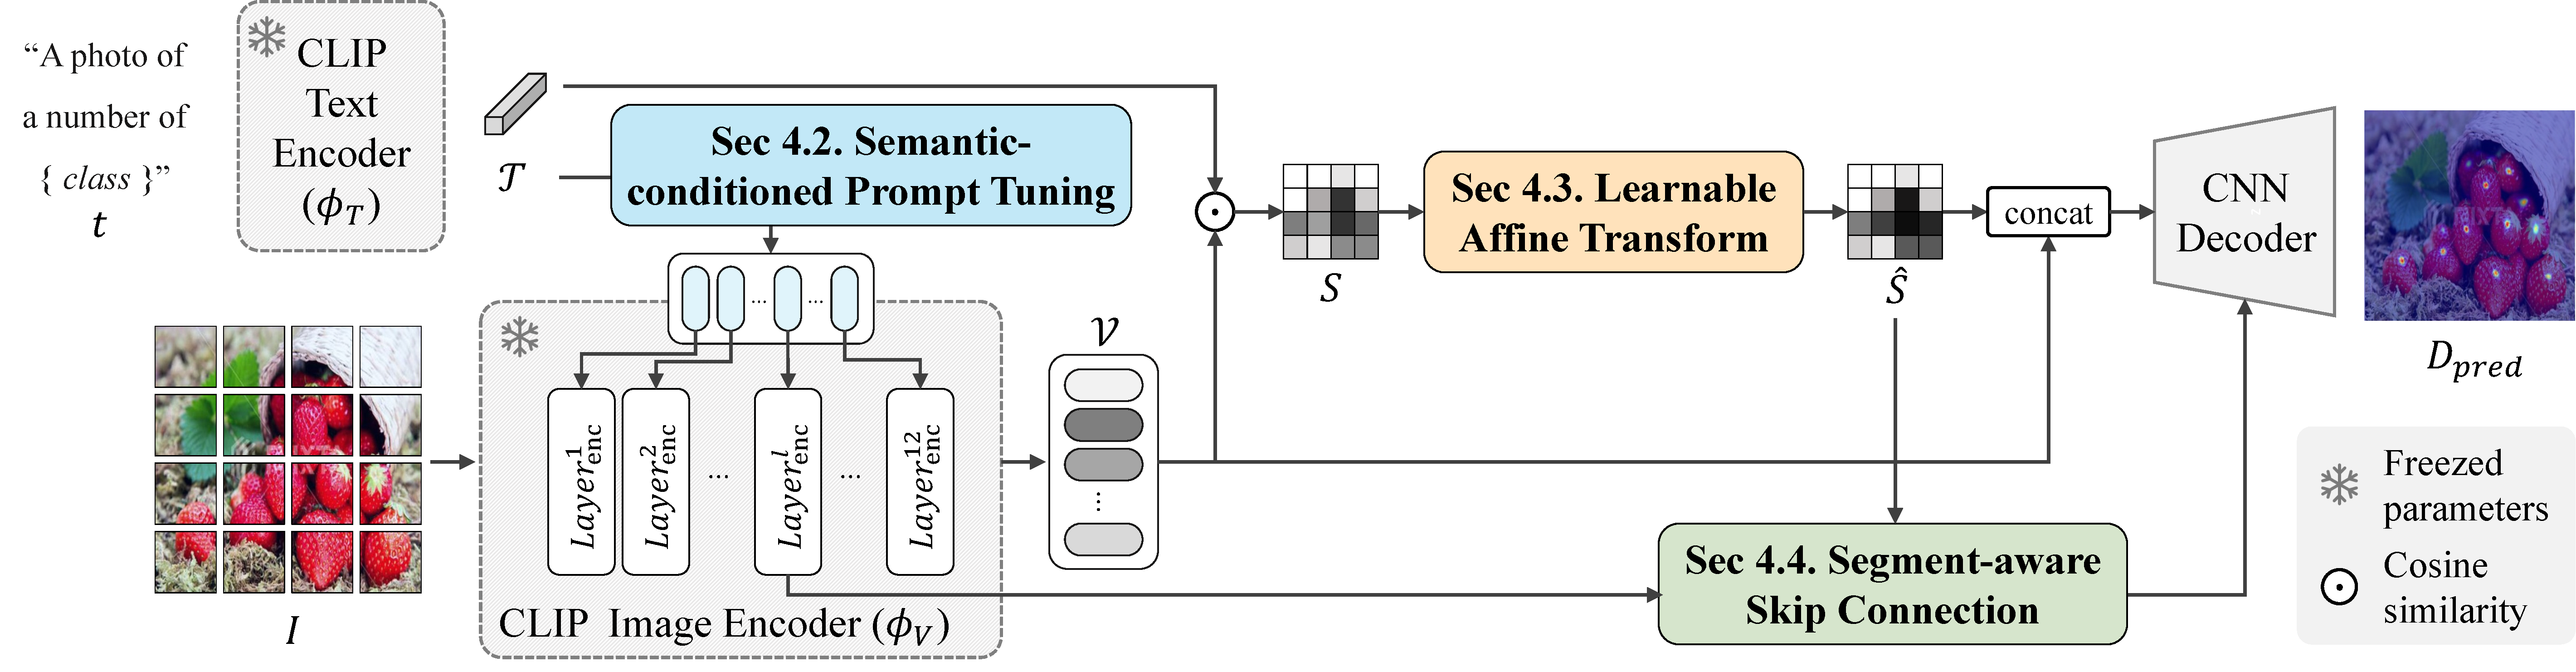
\includegraphics[width=\linewidth]{figs/VLCounter_overview.pdf}
    \end{center}
    \caption{
        Overview of VLBase and VLCounter: each without and with colored components.
        The end-to-end baseline, VLBase, employs CLIP encoders to extract both image and text embeddings. 
        Then, the decoder processes the image-text similarity map along with visual embeddings to count the number of specified objects.
        With three colored modules, VLCounter leverages the generalization capability of VLBase to be tailored for object counting.
    }
    \label{fig:VLCounter_overview}
\end{figure*}



\section{Preliminaries}
\subsection{Problem Formulation: ZSOC}
\label{Method:Formulation}
ZSOC aims to predict the density map $D\in \mathbb{R}^{H\times W \times 1}$ for image $I\in \mathbb{R}^{H\times W \times3}$ that belongs to unseen classes $C^u$~($f:(I, C^u)\mapsto D$) without any visual exemplar clues.
In the training stage, the model is trained with $\mathcal{D}_\text{train} = \{(I_i, C^s_i, D_i)\}_{i=1}^{i=\mathbb{N}}$ where $C^s_i$ denotes the seen class names during training.
Then in the testing stage, the model is to yield a density map for $\mathcal{D}_\text{test}=\{(I_i, C^u_i, D_i)\}_{i=\mathbb{N}+1}^{i=\mathbb{M}}$, where $C^s \cap C^u=\varnothing$.


\subsection{Overview of CLIP}
\label{Method:preliminaries}
This section introduces the underlying motivation behind our proposed method.
CLIP is composed of two encoders: an image encoder $\phi_{V}(\cdot)$ and a text encoder $\phi_{T}(\cdot)$.
The text encoder takes prompted class name~$t$ e.g., \textit{A photo of [$kiwi$]} and produces a semantic embedding $\mathcal{T} \in \mathbb{R}^{1 \times d}$ where $d$ represents an embedding dimension.
The image encoder takes a learnable class token $[cls]$ along with embedded patch sequences $V$ as inputs and encodes global and local semantics in the class token $[cls]$ and patch tokens $\mathcal{V}$ respectively.
Note that $V = [v_1, v_2,...,v_N] \in \mathbb{R}^{N \times (P^2 \cdot d)}$ where $N$ is the number of embedded patches, and $(P \cdot P)$ is the resolution of each patch.
Formally, this process can be expressed as follows:
\begin{equation}
    \mathcal{T} = \phi_{T}(t); \quad\quad[\text{ }[cls],\mathcal{V}\text{ }] = \phi_{V}([\text{ }[cls], V\text{ }]).
\end{equation}
These encoders are trained collaboratively to map $\mathcal{T}$ and $[cls]$ into a shared representation space.


Recently, there exist studies suggesting the implicit localization capability of CLIP, where each patch embedding preserves local image semantics~\cite{2022maskclip, li2023clipsurgery}.
And this property, coupled with the powerful image-text joint embedding space of CLIP, has provided a clear motivation for utilizing CLIP as a robust tool for zero-shot segmentation~(localization).~\cite{li2022languagedriven, rao2022denseclip, luddecke2022image}.
Taking similar inspiration yet focused on object counting, we aim to leverage the implicit localization capability of CLIP to achieve precise and efficient object counting in an end-to-end manner.



